\chapter{Esecuzione}
\label{ch:results}
Qui vengono confrontati i due algoritmi REPTree e RIPPER/JRip. Entrambi hanno sfruttato una \textit{10-fold cross validation}.

\section{Risultati su \texttt{German Credit}}

\normalsize L'esecuzione ha coinvolto 900 istanze di training e 100 istanze di testing.

\begin{mdframed}[frametitle=Esecuzione REPTree]
	\footnotesize\verbatiminput{results/reptree/german_credit.reptree}
\end{mdframed}

%\begin{table}[htbp]
\scriptsize
\begin{adjustbox}{center}
\begin{tabular}{|l|r|r|r|r|r|r|r|r|r|r|}
\hline
\diagbox[width=11em]{\emph{Measures}}{\emph{Key Fold}} & 1 & 2 & 3 & 4 & 5 & 6 & 7 & 8 & 9 & 10 \\ \hline
Number correct & 71 & 74 & 73 & 71 & 66 & 72 & 74 & 66 & 75 & 76 \\ \hline
Number incorrect & 29 & 26 & 27 & 29 & 34 & 28 & 26 & 34 & 25 & 24 \\ \hline
Number unclassified & 0 & 0 & 0 & 0 & 0 & 0 & 0 & 0 & 0 & 0 \\ \hline
Percent correct & 71 & 74 & 73 & 71 & 66 & 72 & 74 & 66 & 75 & 76 \\ \hline
Percent incorrect & 29 & 26 & 27 & 29 & 34 & 28 & 26 & 34 & 25 & 24 \\ \hline
Percent unclassified & 0 & 0 & 0 & 0 & 0 & 0 & 0 & 0 & 0 & 0 \\ \hline
True positive rate & 0.814286 & 0.928571 & 0.857143 & 0.842857 & 0.785714 & 0.928571 & 0.885714 & 0.742857 & 0.942857 & 0.857143 \\ \hline
Num true positives & 57 & 65 & 60 & 59 & 55 & 65 & 62 & 52 & 66 & 60 \\ \hline
False positive rate & 0.533333 & 0.7 & 0.566667 & 0.6 & 0.633333 & 0.766667 & 0.6 & 0.533333 & 0.7 & 0.466667 \\ \hline
Num false positives & 16 & 21 & 17 & 18 & 19 & 23 & 18 & 16 & 21 & 14 \\ \hline
True negative rate & 0.466667 & 0.3 & 0.433333 & 0.4 & 0.366667 & 0.233333 & 0.4 & 0.466667 & 0.3 & 0.533333 \\ \hline
Num true negatives & 14 & 9 & 13 & 12 & 11 & 7 & 12 & 14 & 9 & 16 \\ \hline
False negative rate & 0.185714 & 0.071429 & 0.142857 & 0.157143 & 0.214286 & 0.071429 & 0.114286 & 0.257143 & 0.057143 & 0.142857 \\ \hline
Num false negatives & 13 & 5 & 10 & 11 & 15 & 5 & 8 & 18 & 4 & 10 \\ \hline
\textbf{Precision} & 0.780822 & 0.755814 & 0.779221 & 0.766234 & 0.743243 & 0.738636 & 775 & 0.764706 & 0.758621 & 0.810811 \\ \hline
\textbf{Recall} & 0.814286 & 0.928571 & 0.857143 & 0.842857 & 0.785714 & 0.928571 & 0.885714 & 0.742857 & 0.942857 & 0.857143 \\ \hline
\textbf{F-measure} & 0.797203 & 0.833333 & 0.816327 & 0.802721 & 0.763889 & 0.822785 & 0.826667 & 0.753623 & 0.840764 & 0.833333 \\ \hline\end{tabular}
\end{adjustbox}
\caption{Risultati della 10-fold CV per REPTree}
\label{}
\end{table}



\begin{sidewaysfigure}
	\thisfloatpagestyle{empty}
	\makebox[\textwidth]{
\includegraphics[width=1.4\textwidth, height=.4\textheight]{results/reptree/gc.pdf}}
	\caption{Modello di REPTree}
\end{sidewaysfigure}

\pagebreak

\begin{mdframed}[frametitle=Esecuzione JRip]
	\footnotesize\verbatiminput{results/jrip/german_credit.jrip}
\end{mdframed}

%\begin{table}[htbp]
\scriptsize
\begin{adjustbox}{center}
\begin{tabular}{|l|r|r|r|r|r|r|r|r|r|r|}
\hline
\diagbox[width=11em]{\emph{Measures}}{\emph{Key Fold}} & 1 & 2 & 3 & 4 & 5 & 6 & 7 & 8 & 9 & 10 \\ \hline
Number correct & 71 & 74 & 73 & 71 & 66 & 72 & 74 & 66 & 75 & 76 \\ \hline
Number incorrect & 29 & 26 & 27 & 29 & 34 & 28 & 26 & 34 & 25 & 24 \\ \hline
Number unclassified & 0 & 0 & 0 & 0 & 0 & 0 & 0 & 0 & 0 & 0 \\ \hline
Percent correct & 71 & 74 & 73 & 71 & 66 & 72 & 74 & 66 & 75 & 76 \\ \hline
Percent incorrect & 29 & 26 & 27 & 29 & 34 & 28 & 26 & 34 & 25 & 24 \\ \hline
Percent unclassified & 0 & 0 & 0 & 0 & 0 & 0 & 0 & 0 & 0 & 0 \\ \hline
True positive rate & 0.814286 & 0.928571 & 0.857143 & 0.842857 & 0.785714 & 0.928571 & 0.885714 & 0.742857 & 0.942857 & 0.857143 \\ \hline
Num true positives & 57 & 65 & 60 & 59 & 55 & 65 & 62 & 52 & 66 & 60 \\ \hline
False positive rate & 0.533333 & 0.7 & 0.566667 & 0.6 & 0.633333 & 0.766667 & 0.6 & 0.533333 & 0.7 & 0.466667 \\ \hline
Num false positives & 16 & 21 & 17 & 18 & 19 & 23 & 18 & 16 & 21 & 14 \\ \hline
True negative rate & 0.466667 & 0.3 & 0.433333 & 0.4 & 0.366667 & 0.233333 & 0.4 & 0.466667 & 0.3 & 0.533333 \\ \hline
Num true negatives & 14 & 9 & 13 & 12 & 11 & 7 & 12 & 14 & 9 & 16 \\ \hline
False negative rate & 0.185714 & 0.071429 & 0.142857 & 0.157143 & 0.214286 & 0.071429 & 0.114286 & 0.257143 & 0.057143 & 0.142857 \\ \hline
Num false negatives & 13 & 5 & 10 & 11 & 15 & 5 & 8 & 18 & 4 & 10 \\ \hline
\textbf{Precision} & 0.780822 & 0.755814 & 0.779221 & 0.766234 & 0.743243 & 0.738636 & 775 & 0.764706 & 0.758621 & 0.810811 \\ \hline
\textbf{Recall} & 0.814286 & 0.928571 & 0.857143 & 0.842857 & 0.785714 & 0.928571 & 0.885714 & 0.742857 & 0.942857 & 0.857143 \\ \hline
\textbf{F-measure} & 0.797203 & 0.833333 & 0.816327 & 0.802721 & 0.763889 & 0.822785 & 0.826667 & 0.753623 & 0.840764 & 0.833333 \\ \hline
\end{tabular}
\end{adjustbox}
\caption{Risultati della 10-fold CV per JRip}
\label{}
\end{table}


\noindent
\normalsize Regole:
\footnotesize\input{results/jrip/german_credit.list.rules}

\pagebreak

\section{Risultati su \texttt{Image Segmentation}}

\normalsize L'esecuzione ha coinvolto 2079 istanze di training e 231 istanze di testing.

\begin{mdframed}[frametitle=Esecuzione REPTree]
	\scriptsize\verbatiminput{results/reptree/segment.reptree}
\end{mdframed}

%\begin{table}[htbp]
\scriptsize
\begin{adjustbox}{center}
\begin{tabular}{|l|r|r|r|r|r|r|r|r|r|r|}
\hline
\diagbox[width=11em]{\emph{Measures}}{\emph{Key Fold}} & 1 & 2 & 3 & 4 & 5 & 6 & 7 & 8 & 9 & 10 \\ \hline
Number correct & 220 & 218 & 216 & 219 & 217 & 218 & 220 & 225 & 220 & 223 \\ \hline
Number incorrect & 11 & 13 & 15 & 12 & 14 & 13 & 11 & 6 & 11 & 8 \\ \hline
Number unclassified & 0 & 0 & 0 & 0 & 0 & 0 & 0 & 0 & 0 & 0 \\ \hline
Percent correct & 95.238095 & 94.372294 & 93.506494 & 94.805195 & 93.939394 & 94.372294 & 95.238095 & 97.402597 & 95.238095 & 96.536797 \\ \hline
Percent incorrect & 4.761905 & 5.627706 & 6.493506 & 5.194805 & 6.060606 & 5.627706 & 4.761905 & 2.597403 & 4.761905 & 3.463203 \\ \hline
Percent unclassified & 0 & 0 & 0 & 0 & 0 & 0 & 0 & 0 & 0 & 0 \\ \hline
True positive rate & 0.939394 & 1 & 1 & 1 & 0.939394 & 0.939394 & 0.969697 & 0.939394 & 1 & 1 \\ \hline
Num true positives & 31 & 33 & 33 & 33 & 31 & 31 & 32 & 31 & 33 & 33 \\ \hline
False positive rate & 0.005051 & 0 & 0 & 0.005051 & 0.005051 & 0.015152 & 0 & 0.005051 & 0.015152 & 0.015152 \\ \hline
Num false positives & 1 & 0 & 0 & 1 & 1 & 3 & 0 & 1 & 3 & 3 \\ \hline
True negative rate & 0.994949 & 1 & 1 & 0.994949 & 0.994949 & 0.984848 & 1 & 0.994949 & 0.984848 & 0.984848 \\ \hline
Num true negatives & 197 & 198 & 198 & 197 & 197 & 195 & 198 & 197 & 195 & 195 \\ \hline
False negative rate & 0.060606 & 0 & 0 & 0 & 0.060606 & 0.060606 & 0.030303 & 0.060606 & 0 & 0 \\ \hline
Num false negatives & 2 & 0 & 0 & 0 & 2 & 2 & 1 & 2 & 0 & 0 \\ \hline
\textbf{Precision} & 0.96875 & 1 & 1 & 0.970588 & 0.96875 & 0.911765 & 1 & 0.96875 & 0.916667 & 0.916667 \\ \hline
\textbf{Recall} & 0.939394 & 1 & 1 & 1 & 0.939394 & 0.939394 & 0.969697 & 0.939394 & 1 & 1 \\ \hline
\textbf{F-measure} & 0.953846 & 1 & 1 & 0.985075 & 0.953846 & 0.925373 & 0.984615 & 0.953846 & 0.956522 & 0.956522 \\ \hline
\end{tabular}
\end{adjustbox}
\caption{Risultati della 10-fold CV per REPTree}
\label{}
\end{table}



\begin{figure}[htb]
	\makebox[\textwidth]{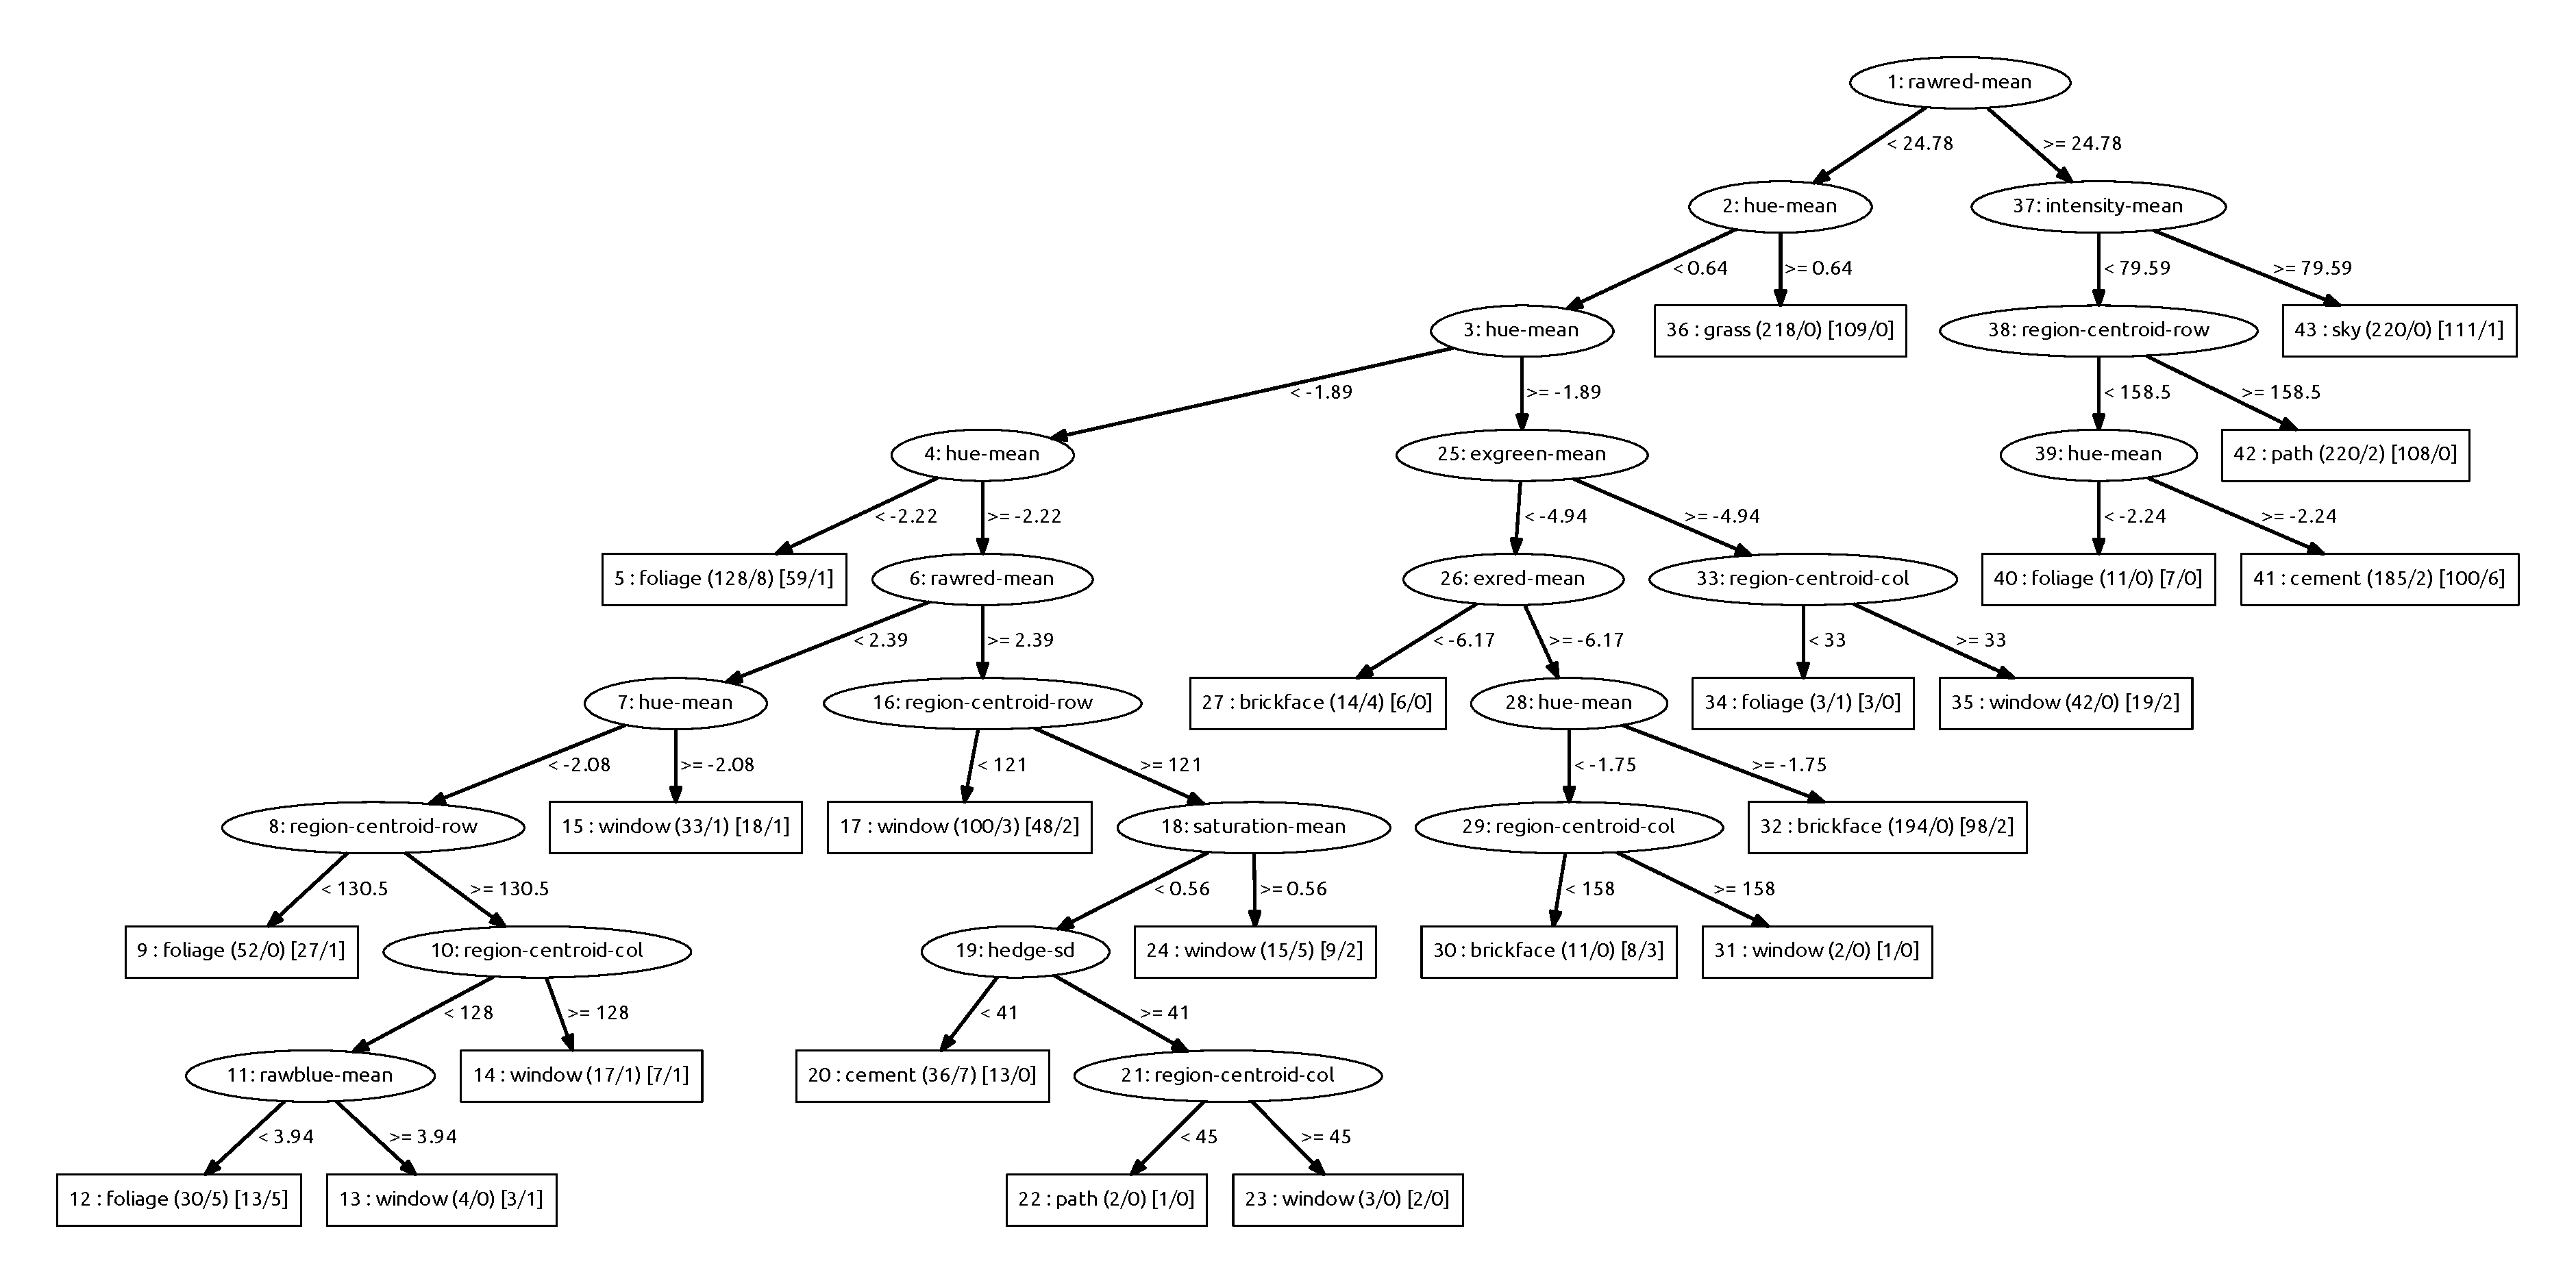
\includegraphics[width=1.55\textwidth]{results/reptree/segment.pdf}}
	\caption{Modello di REPTree}
\end{figure}

\begin{mdframed}[frametitle=Esecuzione JRip]
	\scriptsize\verbatiminput{results/jrip/segment.jrip}
\end{mdframed}

%\begin{table}[htbp]
	\scriptsize
	\begin{adjustbox}{center}
		\begin{tabular}{|l|r|r|r|r|r|r|r|r|r|r|}
		\hline
		\diagbox[width=11em]{\emph{Measures}}{\emph{Key Fold}} & 1 & 2 & 3 & 4 & 5 & 6 & 7 & 8 & 9 & 10 \\ \hline
		Number correct & 222 & 216 & 223 & 219 & 218 & 221 & 220 & 221 & 221 & 223 \\ \hline
		Number incorrect & 9 & 15 & 8 & 12 & 13 & 10 & 11 & 10 & 10 & 8 \\ \hline
		Number unclassified & 0 & 0 & 0 & 0 & 0 & 0 & 0 & 0 & 0 & 0 \\ \hline
		Percent correct & 96.103896 & 93.506494 & 96.536797 & 94.805195 & 94.372294 & 95.670996 & 95.238095 & 95.670996 & 95.670996 & 96.536797 \\ \hline
		Percent incorrect & 3.896104 & 6.493506 & 3.463203 & 5.194805 & 5.627706 & 4.329004 & 4.761905 & 4.329004 & 4.329004 & 3.463203 \\ \hline
		Percent unclassified & 0 & 0 & 0 & 0 & 0 & 0 & 0 & 0 & 0 & 0 \\ \hline
		True positive rate & 0.969697 & 1 & 1 & 0.969697 & 0.969697 & 0.969697 & 0.969697 & 1 & 1 & 0.969697 \\ \hline
		Num true positives & 32 & 33 & 33 & 32 & 32 & 32 & 32 & 33 & 33 & 32 \\ \hline
		False positive rate & 0.005051 & 0.005051 & 0.005051 & 0 & 0.010101 & 0 & 0.005051 & 0.010101 & 0.005051 & 0.005051 \\ \hline
		Num false positives & 1 & 1 & 1 & 0 & 2 & 0 & 1 & 2 & 1 & 1 \\ \hline
		True negative rate & 0.994949 & 0.994949 & 0.994949 & 1 & 0.989899 & 1 & 0.994949 & 0.989899 & 0.994949 & 0.994949 \\ \hline
		Num true negatives & 197 & 197 & 197 & 198 & 196 & 198 & 197 & 196 & 197 & 197 \\ \hline
		False negative rate & 0.030303 & 0 & 0 & 0.030303 & 0.030303 & 0.030303 & 0.030303 & 0 & 0 & 0.030303 \\ \hline
		Num false negatives & 1 & 0 & 0 & 1 & 1 & 1 & 1 & 0 & 0 & 1 \\ \hline
		\textbf{Precision} & 0.969697 & 0.970588 & 0.970588 & 1 & 0.941176 & 1 & 0.969697 & 0.942857 & 0.970588 & 0.969697 \\ \hline
		\textbf{Recall} & 0.969697 & 1 & 1 & 0.969697 & 0.969697 & 0.969697 & 0.969697 & 1 & 1 & 0.969697 \\ \hline
		\textbf{F-measure} & 0.969697 & 0.985075 & 0.985075 & 0.984615 & 0.955224 & 0.984615 & 0.969697 & 0.970588 & 0.985075 & 0.969697 \\ \hline
	\end{tabular}
\end{adjustbox}
	\caption{Risultati della 10-fold CV per JRip}
	\label{}
\end{table}


\noindent
\normalsize Regole:
\scriptsize\input{results/jrip/segment.list.rules}

\pagebreak

\section{Risultati su \texttt{Vehicle Silhouettes}}

\normalsize L'esecuzione ha coinvolto 761 istanze di training e 85 istanze di testing.

\begin{mdframed}[frametitle=Esecuzione REPTree]
	\scriptsize\verbatiminput{results/reptree/vehicle.reptree}
\end{mdframed}

%\begin{table}[htbp]
\scriptsize
\begin{adjustbox}{center}
\begin{tabular}{|l|r|r|r|r|r|r|r|r|r|r|}
\hline
\diagbox[width=11em]{\emph{Measures}}{\emph{Key Fold}} & 1 & 2 & 3 & 4 & 5 & 6 & 7 & 8 & 9 & 10 \\ \hline
Number correct & 55 & 64 & 66 & 62 & 58 & 64 & 57 & 58 & 63 & 65 \\ \hline
Number incorrect & 30 & 21 & 19 & 23 & 27 & 21 & 27 & 26 & 21 & 19 \\ \hline
Number unclassified & 0 & 0 & 0 & 0 & 0 & 0 & 0 & 0 & 0 & 0 \\ \hline
Percent correct & 64.705882 & 75.294118 & 77.647059 & 72.941176 & 68.235294 & 75.294118 & 67.857143 & 69.047619 & 75 & 77.380952 \\ \hline
Percent incorrect & 35.294118 & 24.705882 & 22.352941 & 27.058824 & 31.764706 & 24.705882 & 32.142857 & 30.952381 & 25 & 22.619048 \\ \hline
Percent unclassified & 0 & 0 & 0 & 0 & 0 & 0 & 0 & 0 & 0 & 0 \\ \hline
True positive rate & 0.380952 & 0.619048 & 0.714286 & 0.761905 & 0.619048 & 0.428571 & 0.47619 & 0.454545 & 0.681818 & 0.619048 \\ \hline
Num true positives & 8 & 13 & 15 & 16 & 13 & 9 & 10 & 10 & 15 & 13 \\ \hline
False positive rate & 0.15625 & 0.140625 & 0.109375 & 0.21875 & 0.171875 & 0.046875 & 0.15873 & 0.145161 & 0.129032 & 0.095238 \\ \hline
Num false positives & 10 & 9 & 7 & 14 & 11 & 3 & 10 & 9 & 8 & 6 \\ \hline
True negative rate & 0.84375 & 0.859375 & 0.890625 & 0.78125 & 0.828125 & 0.953125 & 0.84127 & 0.854839 & 0.870968 & 0.904762 \\ \hline
Num true negatives & 54 & 55 & 57 & 50 & 53 & 61 & 53 & 53 & 54 & 57 \\ \hline
False negative rate & 0.619048 & 0.380952 & 0.285714 & 0.238095 & 0.380952 & 0.571429 & 0.52381 & 0.545455 & 0.318182 & 0.380952 \\ \hline
Num false negatives & 13 & 8 & 6 & 5 & 8 & 12 & 11 & 12 & 7 & 8 \\ \hline
\textbf{Precision} & 0.444444 & 0.590909 & 0.681818 & 0.533333 & 0.541667 & 0.75 & 0.5 & 0.526316 & 0.652174 & 0.684211 \\ \hline
\textbf{Recall} & 0.380952 & 0.619048 & 0.714286 & 0.761905 & 0.619048 & 0.428571 & 0.47619 & 0.454545 & 0.681818 & 0.619048 \\ \hline
\textbf{F-measure} & 0.410256 & 0.604651 & 0.697674 & 0.627451 & 0.577778 & 0.545455 & 0.487805 & 0.487805 & 0.666667 & 0.65 \\ \hline
\end{tabular}
\end{adjustbox}
\caption{Risultati della 10-fold CV per REPTree}
\label{}
\end{table}



\begin{figure}[htb]
	\makebox[\textwidth]{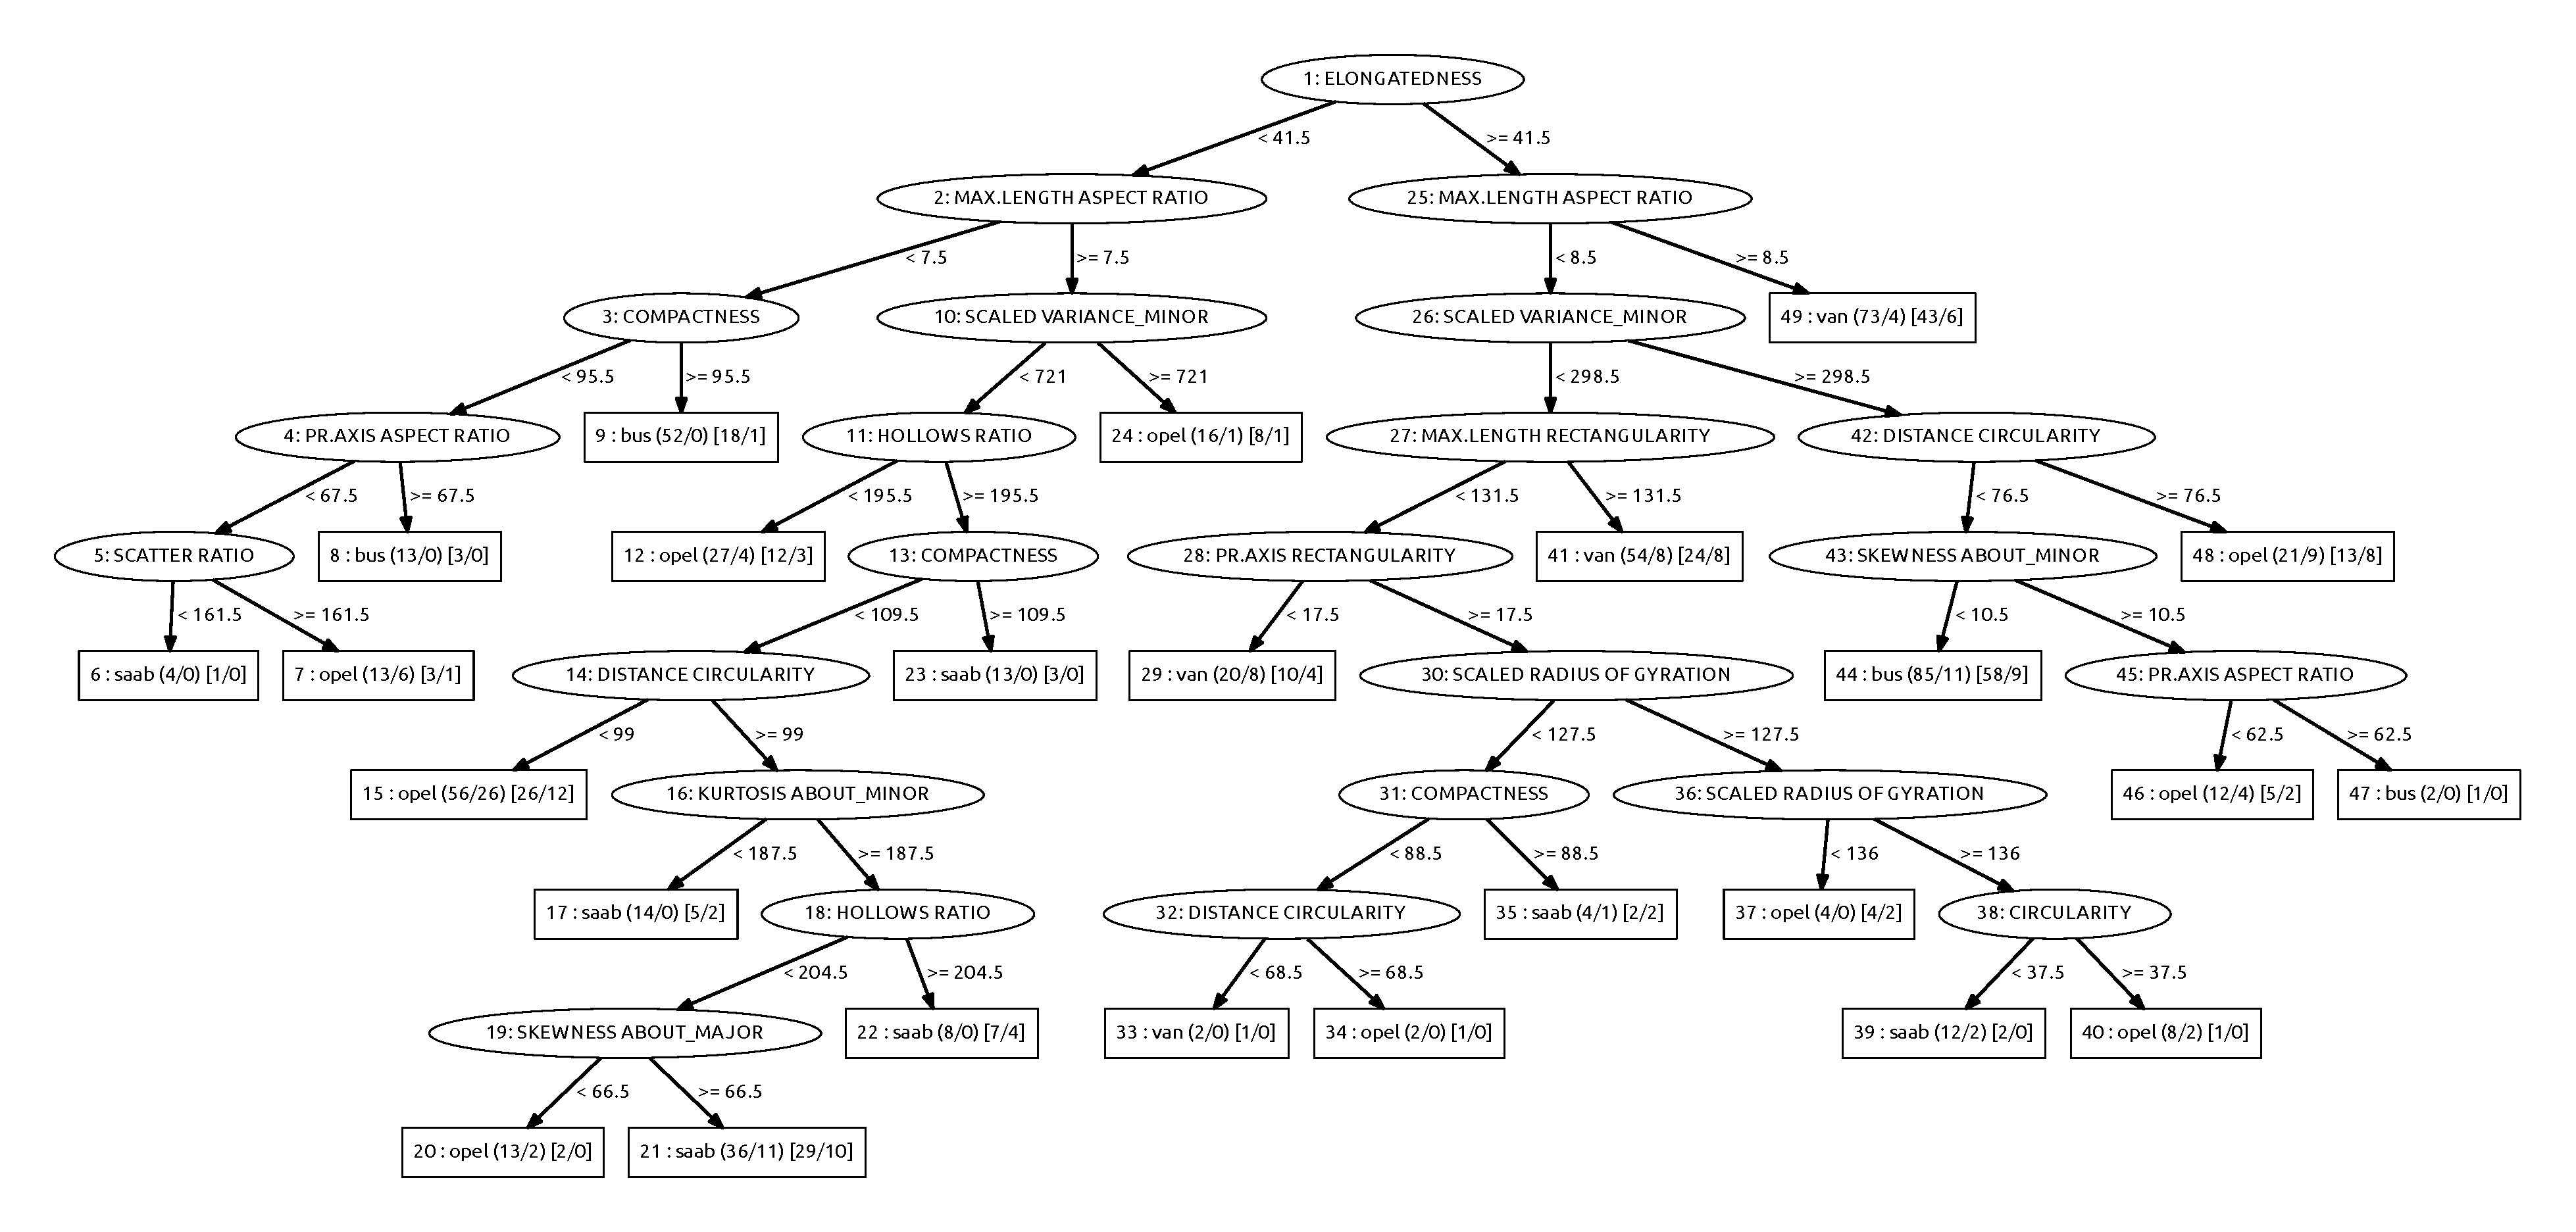
\includegraphics[width=1.55\textwidth]{results/reptree/vehicle.pdf}}
	\caption{Modello di REPTree}
\end{figure}

\begin{mdframed}[frametitle=Esecuzione JRip]
	\scriptsize\verbatiminput{results/jrip/vehicle.jrip}
\end{mdframed}

%\begin{table}[htbp]
\scriptsize
\begin{adjustbox}{center}
\begin{tabular}{|l|r|r|r|r|r|r|r|r|r|r|}
\hline
\diagbox[width=11em]{\emph{Measures}}{\emph{Key Fold}} & 1 & 2 & 3 & 4 & 5 & 6 & 7 & 8 & 9 & 10 \\ \hline
Number correct & 51 & 66 & 54 & 57 & 58 & 59 & 54 & 60 & 58 & 67 \\ \hline
Number incorrect & 34 & 19 & 31 & 28 & 27 & 26 & 30 & 24 & 26 & 17 \\ \hline
Number unclassified & 0 & 0 & 0 & 0 & 0 & 0 & 0 & 0 & 0 & 0 \\ \hline
Percent correct & 60 & 77.647059 & 63.529412 & 67.058824 & 68.235294 & 69.411765 & 64.285714 & 71.428571 & 69.047619 & 79.761905 \\ \hline
Percent incorrect & 40 & 22.352941 & 36.470588 & 32.941176 & 31.764706 & 30.588235 & 35.714286 & 28.571429 & 30.952381 & 20.238095 \\ \hline
Percent unclassified & 0 & 0 & 0 & 0 & 0 & 0 & 0 & 0 & 0 & 0 \\ \hline
True positive rate & 0.095238 & 0.666667 & 0.428571 & 0.285714 & 0.571429 & 0.666667 & 0.52381 & 0.545455 & 0.409091 & 0.619048 \\ \hline
Num true positives & 2 & 14 & 9 & 6 & 12 & 14 & 11 & 12 & 9 & 13 \\ \hline
False positive rate & 0.046875 & 0.09375 & 0.15625 & 125 & 0.140625 & 0.1875 & 0.190476 & 0.096774 & 0.145161 & 0.079365 \\ \hline
Num false positives & 3 & 6 & 10 & 8 & 9 & 12 & 12 & 6 & 9 & 5 \\ \hline
True negative rate & 0.953125 & 0.90625 & 0.84375 & 875 & 0.859375 & 0.8125 & 0.809524 & 0.903226 & 0.854839 & 0.920635 \\ \hline
Num true negatives & 61 & 58 & 54 & 56 & 55 & 52 & 51 & 56 & 53 & 58 \\ \hline
False negative rate & 0.904762 & 0.333333 & 0.571429 & 0.714286 & 0.428571 & 0.333333 & 0.47619 & 0.454545 & 0.590909 & 0.380952 \\ \hline
Num false negatives & 19 & 7 & 12 & 15 & 9 & 7 & 10 & 10 & 13 & 8 \\ \hline
\textbf{Precision} & 0.4 & 0.7 & 0.473684 & 0.428571 & 0.571429 & 0.538462 & 0.478261 & 0.666667 & 0.5 & 0.722222 \\ \hline
\textbf{Recall} & 0.095238 & 0.666667 & 0.428571 & 0.285714 & 0.571429 & 0.666667 & 0.52381 & 0.545455 & 0.409091 & 0.619048 \\ \hline
\textbf{F-measure} & 0.153846 & 0.682927 & 0.45 & 0.342857 & 0.571429 & 0.595745 & 0.5 & 0.6 & 0.45 & 0.666667 \\ \hline
\end{tabular}
\end{adjustbox}
\caption{Risultati della 10-fold CV per JRip}
\label{}
\end{table}



\noindent
\normalsize Regole:
\scriptsize\input{results/jrip/vehicle.list.rules}

\pagebreak

\section{Risultati su \texttt{Wisconsin Breast Cancer}}

\normalsize L'esecuzione ha coinvolto 629 istanze di training e 70 istanze di testing.

\begin{mdframed}[frametitle=Esecuzione REPTree]
	\footnotesize\verbatiminput{results/reptree/wisconsin_breast_cancer.reptree}
\end{mdframed}

%\begin{table}[htbp]
\scriptsize
\begin{adjustbox}{center}
\begin{tabular}{|l|r|r|r|r|r|r|r|r|r|r|}
\hline
\diagbox[width=11em]{\emph{Measures}}{\emph{Key Fold}} & 1 & 2 & 3 & 4 & 5 & 6 & 7 & 8 & 9 & 10 \\ \hline
Number correct & 69 & 63 & 67 & 62 & 64 & 69 & 66 & 65 & 66 & 65 \\ \hline
Number incorrect & 1 & 7 & 3 & 8 & 6 & 1 & 4 & 5 & 4 & 4 \\ \hline
Number unclassified & 0 & 0 & 0 & 0 & 0 & 0 & 0 & 0 & 0 & 0 \\ \hline
Percent correct & 98.571429 & 90 & 95.714286 & 88.571429 & 91.428571 & 98.571429 & 94.285714 & 92.857143 & 94.285714 & 94.202899 \\ \hline
Percent incorrect & 1.428571 & 10 & 4.285714 & 11.428571 & 8.571429 & 1.428571 & 5.714286 & 7.142857 & 5.714286 & 5.797101 \\ \hline
Percent unclassified & 0 & 0 & 0 & 0 & 0 & 0 & 0 & 0 & 0 & 0 \\ \hline
True positive rate & 0.978261 & 0.978261 & 0.956522 & 0.891304 & 0.869565 & 0.978261 & 0.934783 & 0.934783 & 0.955556 & 0.933333 \\ \hline
Num true positives & 45 & 45 & 44 & 41 & 40 & 45 & 43 & 43 & 43 & 42 \\ \hline
False positive rate & 0 & 0.25 & 0.041667 & 125 & 0 & 0 & 0.041667 & 0.083333 & 0.08 & 0.041667 \\ \hline
Num false positives & 0 & 6 & 1 & 3 & 0 & 0 & 1 & 2 & 2 & 1 \\ \hline
True negative rate & 1 & 0.75 & 0.958333 & 875 & 1 & 1 & 0.958333 & 0.916667 & 0.92 & 0.958333 \\ \hline
Num true negatives & 24 & 18 & 23 & 21 & 24 & 24 & 23 & 22 & 23 & 23 \\ \hline
False negative rate & 0.021739 & 0.021739 & 0.043478 & 0.108696 & 0.130435 & 0.021739 & 0.065217 & 0.065217 & 0.044444 & 0.066667 \\ \hline
Num false negatives & 1 & 1 & 2 & 5 & 6 & 1 & 3 & 3 & 2 & 3 \\ \hline
\textbf{Precision} & 1 & 0.882353 & 0.977778 & 0.931818 & 1 & 1 & 0.977273 & 0.955556 & 0.955556 & 0.976744 \\ \hline
\textbf{Recall} & 0.978261 & 0.978261 & 0.956522 & 0.891304 & 0.869565 & 0.978261 & 0.934783 & 0.934783 & 0.955556 & 0.933333 \\ \hline
\textbf{F-measure} & 0.989011 & 0.927835 & 0.967033 & 0.911111 & 0.930233 & 0.989011 & 0.955556 & 0.945055 & 0.955556 & 0.954545 \\ \hline
\end{tabular}
\end{adjustbox}
\caption{Risultati della 10-fold CV per REPTree}
\label{}
\end{table}



\begin{figure}[htb]
	\makebox[\textwidth]{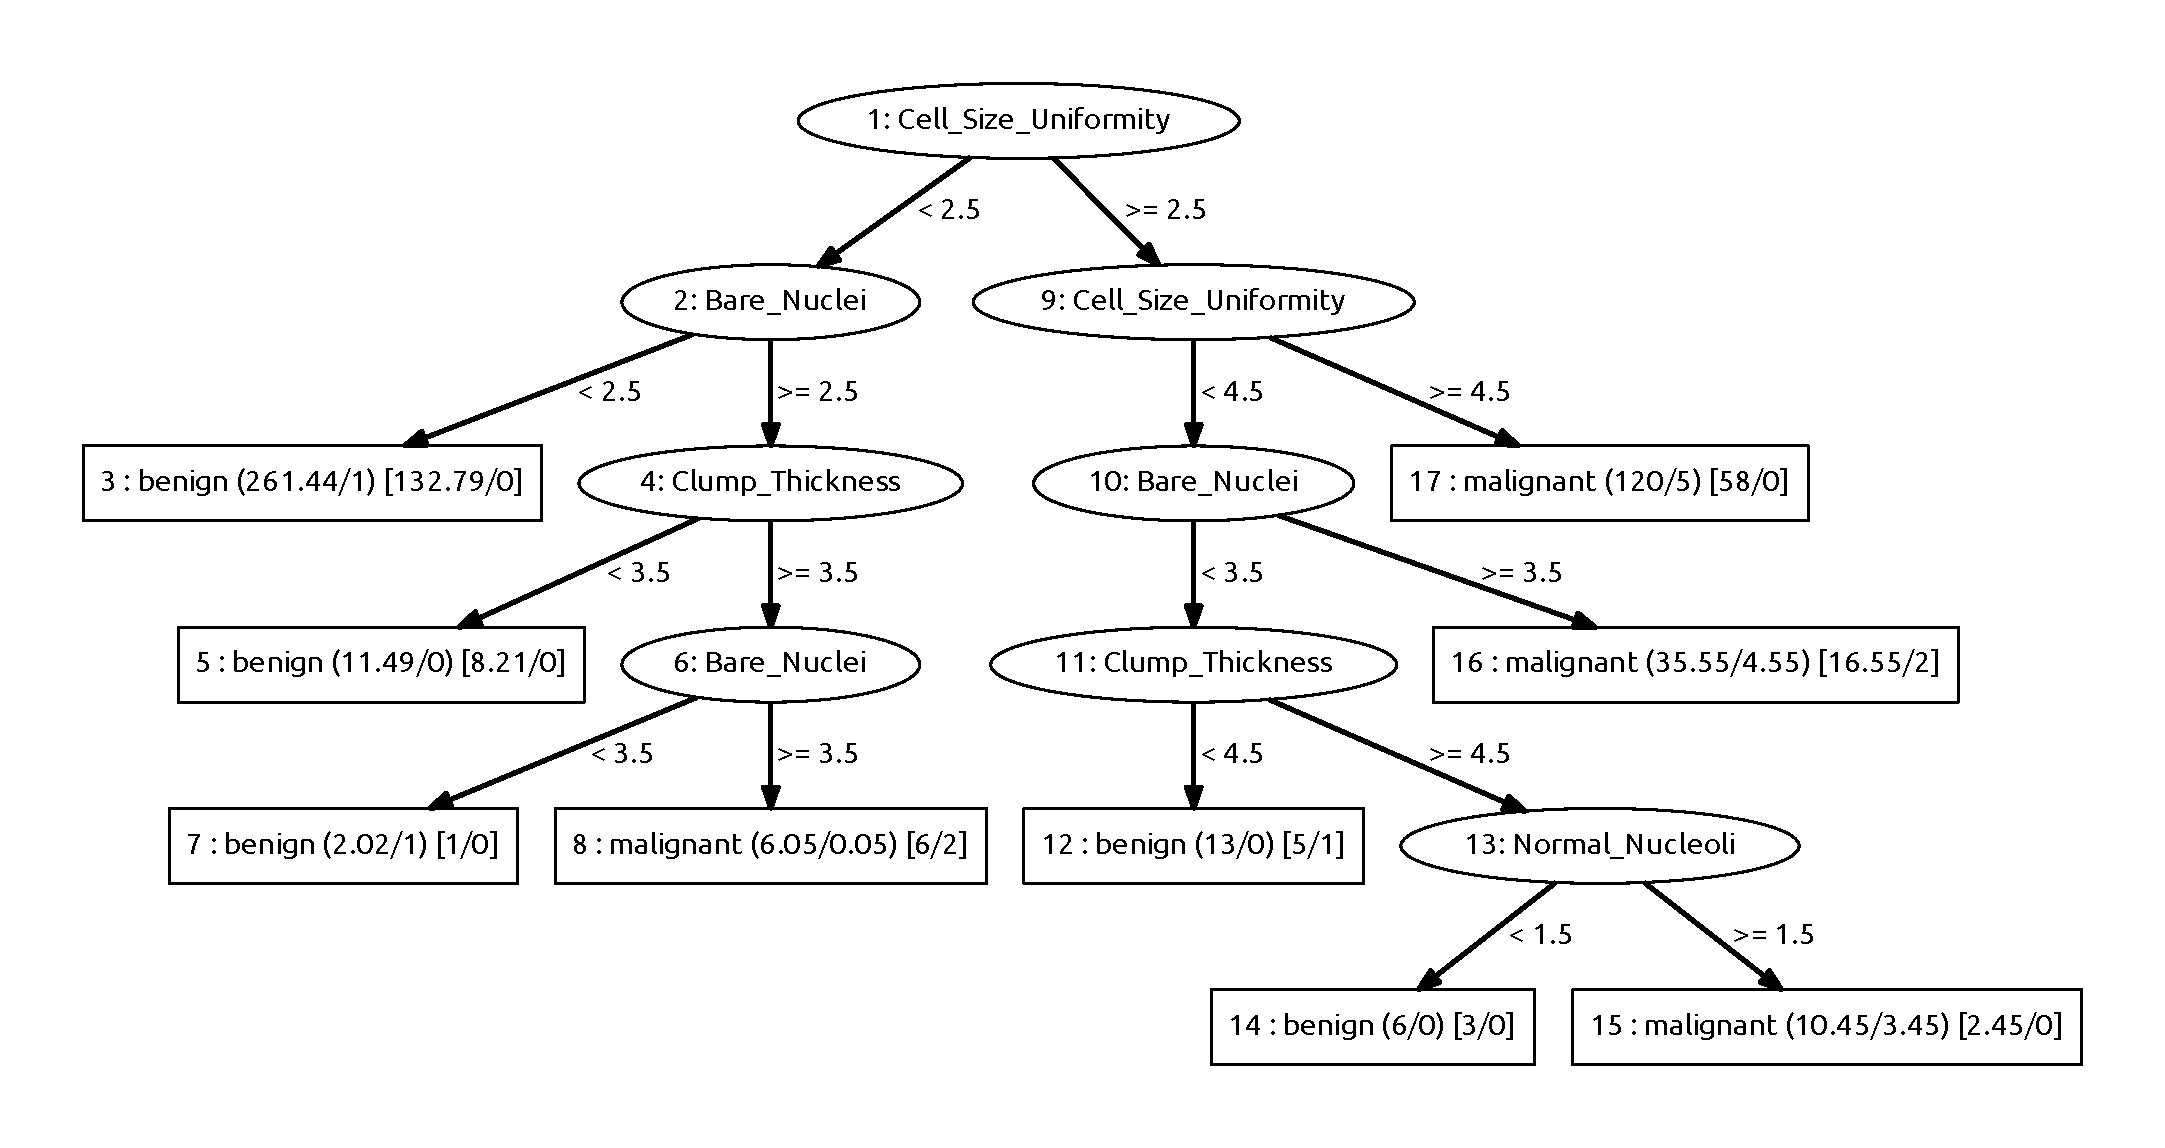
\includegraphics[width=1.55\textwidth]{results/reptree/wisconsin_breast_cancer.pdf}}
	\caption{Modello di REPTree}
\end{figure}

\begin{mdframed}[frametitle=Esecuzione JRip]
	\footnotesize\verbatiminput{results/jrip/wisconsin_breast_cancer.jrip}
\end{mdframed}

%\begin{table}[htbp]
\scriptsize
\begin{adjustbox}{center}
\begin{tabular}{|l|r|r|r|r|r|r|r|r|r|r|}
\hline
\diagbox[width=11em]{\emph{Measures}}{\emph{Key Fold}} & 1 & 2 & 3 & 4 & 5 & 6 & 7 & 8 & 9 & 10 \\ \hline
Number correct & 69 & 64 & 68 & 66 & 64 & 69 & 67 & 68 & 67 & 65 \\ \hline
Number incorrect & 1 & 6 & 2 & 4 & 6 & 1 & 3 & 2 & 3 & 4 \\ \hline
Number unclassified & 0 & 0 & 0 & 0 & 0 & 0 & 0 & 0 & 0 & 0 \\ \hline
Percent correct & 98.571429 & 91.428571 & 97.142857 & 94.285714 & 91.428571 & 98.571429 & 95.714286 & 97.142857 & 95.714286 & 94.202899 \\ \hline
Percent incorrect & 1.428571 & 8.571429 & 2.857143 & 5.714286 & 8.571429 & 1.428571 & 4.285714 & 2.857143 & 4.285714 & 5.797101 \\ \hline
Percent unclassified & 0 & 0 & 0 & 0 & 0 & 0 & 0 & 0 & 0 & 0 \\ \hline
True positive rate & 0.978261 & 0.956522 & 0.956522 & 0.913043 & 0.891304 & 1 & 0.934783 & 0.978261 & 0.977778 & 0.933333 \\ \hline
Num true positives & 45 & 44 & 44 & 42 & 41 & 46 & 43 & 45 & 44 & 42 \\ \hline
False positive rate & 0 & 0.166667 & 0 & 0 & 0.041667 & 0.041667 & 0 & 0.041667 & 0.08 & 0.041667 \\ \hline
Num false positives & 0 & 4 & 0 & 0 & 1 & 1 & 0 & 1 & 2 & 1 \\ \hline
True negative rate & 1 & 0.833333 & 1 & 1 & 0.958333 & 0.958333 & 1 & 0.958333 & 0.92 & 0.958333 \\ \hline
Num true negatives & 24 & 20 & 24 & 24 & 23 & 23 & 24 & 23 & 23 & 23 \\ \hline
False negative rate & 0.021739 & 0.043478 & 0.043478 & 0.086957 & 0.108696 & 0 & 0.065217 & 0.021739 & 0.022222 & 0.066667 \\ \hline
Num false negatives & 1 & 2 & 2 & 4 & 5 & 0 & 3 & 1 & 1 & 3 \\ \hline
\textbf{Precision} & 1 & 0.916667 & 1 & 1 & 0.97619 & 0.978723 & 1 & 0.978261 & 0.956522 & 0.976744 \\ \hline
\textbf{Recall} & 0.978261 & 0.956522 & 0.956522 & 0.913043 & 0.891304 & 1 & 0.934783 & 0.978261 & 0.977778 & 0.933333 \\ \hline
\textbf{F-measure} & 0.989011 & 0.93617 & 0.977778 & 0.954545 & 0.931818 & 0.989247 & 0.966292 & 0.978261 & 0.967033 & 0.954545 \\ \hline
\end{tabular}
\end{adjustbox}
\caption{Risultati della 10-fold CV per JRip}
\label{}
\end{table}



\noindent
\normalsize Regole:
\footnotesize\input{results/jrip/wisconsin_breast_cancer.list.rules}